\documentclass[aspectratio=169,11pt]{beamer}

\usepackage{amsmath,amssymb}
\usepackage{booktabs}
\usepackage{graphicx}
\usepackage{tikz}
\usepackage{pgfplots}
\usetikzlibrary{positioning,fit,arrows.meta,backgrounds}
\pgfplotsset{compat=1.16}

\definecolor{navy}{HTML}{0F2B40}
\definecolor{okorange}{HTML}{E8832A}
\definecolor{okgreen}{HTML}{2F8F5B}
\definecolor{mint}{HTML}{E3F2E9}
\definecolor{peach}{HTML}{FDEFD9}

\newcommand{\IdleShare}{63}
\newcommand{\IdleShareStress}{46}
\newcommand{\NSeeds}{50}
\newcommand{\HeadlineW}{1.5}
\newcommand{\FusedCO}{12.9}
\newcommand{\FusedCOci}{1.2}
\newcommand{\FusedCOStress}{2.4}
\newcommand{\FusedLatCut}{81}
\newcommand{\NetLatCut}{83}
\newcommand{\NetCO}{1.7}
\newcommand{\FusedLatCutStress}{54}
\newcommand{\NetLatCutStress}{56}
\newcommand{\FusedLowW}{5.2}
\newcommand{\EnergyOnlyCO}{7.3}
\newcommand{\FusedDecisionUs}{3.4}
\newcommand{\NSystemsScraped}{1118}
\newcommand{\NSystemsKept}{1115}
\newcommand{\NRowsKept}{12{,}265}
\newcommand{\YearLo}{2007}
\newcommand{\YearHi}{2026}
\newcommand{\MapeXgb}{12.0}
\newcommand{\MapeOracle}{7.7}
\newcommand{\MapePlaceholder}{65}
\newcommand{\MapeTemporal}{26}
\newcommand{\TrainSystems}{800}
\newcommand{\TestSystems}{315}
\newcommand{\SmallIdle}{32}
\newcommand{\SmallHalf}{59}
\newcommand{\SmallPeak}{89}


% ------------------------------------------------------------------ theme
\usefonttheme{professionalfonts}
\setbeamertemplate{navigation symbols}{}
\setbeamercolor{normal text}{fg=navy!90!black}
\setbeamercolor{itemize item}{fg=okorange}
\setbeamercolor{itemize subitem}{fg=okgreen}
\setbeamerfont{itemize/enumerate body}{size=\small}
\setbeamerfont{itemize/enumerate subbody}{size=\footnotesize}
\setbeamertemplate{itemize item}[circle]
\setbeamertemplate{itemize subitem}[circle]
\setbeamertemplate{frametitle}{%
  \vskip0.28cm
  {\color{okorange}\tiny\bfseries\MakeUppercase{\insertframesubtitle}}\par\vskip1pt
  {\color{navy}\Large\bfseries\insertframetitle}\par\vskip3pt
  {\color{okorange}\rule{1.1cm}{1.6pt}}}
\setbeamertemplate{footline}{%
  \begin{tikzpicture}[remember picture, overlay]
    \fill[okorange] (current page.south west) rectangle ++(0.35\paperwidth,0.07);
    \fill[okgreen] ([xshift=0.35\paperwidth]current page.south west) rectangle (current page.south east |- 0,0.07 |- current page.south);
    \node[anchor=south west, font=\sffamily\tiny, text=navy!60] at ([yshift=0.14cm,xshift=0.55cm]current page.south west)
      {OKUBE-ENERGY \ $\bullet$ \ Course project, NITK Surathkal};
    \node[anchor=south east, font=\sffamily\tiny, text=navy!60] at ([yshift=0.14cm,xshift=-0.55cm]current page.south east)
      {\insertframenumber\,/\,\inserttotalframenumber};
  \end{tikzpicture}}
\setlength{\leftmargini}{1.1em}

\newcommand{\chip}[2]{\tikz[baseline=(c.base)]\node[fill=#1, text=white, rounded corners=7pt, inner xsep=6pt, inner ysep=2pt, font=\sffamily\bfseries\tiny](c){\MakeUppercase{#2}};}
\newcommand{\stat}[3]{%
  \begin{tikzpicture}\node[fill=#1, text=white, rounded corners=4pt, inner sep=5pt, align=center, minimum width=#3]{{\Large\bfseries #2}};\end{tikzpicture}}

\title{Okube-Energy}
\author{Sanchit Srisha Udupa (231IT060)\\Aditi Pandey (231IT003)}
\date{October 2026}

\begin{document}

% ------------------------------------------------------------------ 1 title
{\setbeamercolor{background canvas}{bg=navy}
\begin{frame}[plain]
\begin{tikzpicture}[remember picture, overlay]
  \fill[okorange] (current page.north west) rectangle ++(0.12,-\paperheight);
  \node[anchor=north east, inner sep=0.5cm] at (current page.north east) {
\includegraphics[height=2.1cm]{figures/nitk_logo.png}};
\end{tikzpicture}
\vspace{0.9cm}
\begin{flushleft}
{\color{white!70!navy}\scriptsize\bfseries OKUBE-ENERGY \ $\bullet$ \ COURSE PROJECT}\\[10pt]
{\color{white}\fontsize{25}{29}\selectfont\bfseries Fusing Network and Carbon Cost\\in a Custom Container Scheduler}\\[10pt]
{\color{white!80!navy}\small Okube: a Go orchestrator that scores every node on latency and on carbon}\\[8pt]
\chip{navy!60!white}{custom go orchestrator}\ \chip{okorange}{network + carbon}\ \chip{okgreen}{power model from specpower}\\[16pt]
{\color{white}\footnotesize\bfseries Sanchit Srisha Udupa (231IT060) \quad Aditi Pandey (231IT003)}\\[2pt]
{\color{white!75!navy}\scriptsize Guide: Dr.\ Bhawana Rudra \ $\bullet$ \ Department of Information Technology, NIT Karnataka, Surathkal \ $\bullet$ \ October 2026}
\end{flushleft}
\end{frame}}

% ------------------------------------------------------------------ 2 problem
\begin{frame}[t]
\frametitle{Schedulers are blind to two costs}
\framesubtitle{The problem}
\begin{columns}[T]
\begin{column}{0.48\textwidth}
\begin{block}{Network cost}
Dependent services placed far apart pay latency on every call, even when each node is well provisioned.
\end{block}
\end{column}
\begin{column}{0.48\textwidth}
\begin{block}{Carbon cost}
The same task draws different energy on different nodes, and each node's grid has a different carbon intensity.
\end{block}
\end{column}
\end{columns}
\vspace{4pt}
\begin{itemize}
\item The default Kubernetes scheduler ranks nodes by \textbf{resource fit} only.
\item A resource-optimal placement is often neither latency-optimal nor carbon-optimal.
\item Prior work fixes one cost at a time, so the two goals are never traded off in one decision.
\end{itemize}
\vspace{2pt}
\begin{center}
\fbox{\parbox{0.86\textwidth}{\centering\footnotesize\textbf{Question.} Can one scheduler score nodes on network \emph{and} carbon cost, and cut CO$_2$ without giving back the latency win?}}
\end{center}
\end{frame}

% ------------------------------------------------------------------ 3 gap
\begin{frame}[t]
\frametitle{Each prior work covers one piece}
\framesubtitle{Related work and the gap}
\vspace{-8pt}
\begin{center}
\footnotesize
\setlength{\tabcolsep}{4pt}
\begin{tabular}{@{}lccccc@{}}
\toprule
 & Network-aware & Carbon signal & Class-aware & Learned power & Fused + ablations \\
\midrule
Diktyo (Santos et al.)    & \checkmark & $\times$ & $\times$ & $\times$ & $\times$ \\
Piontek et al.            & $\times$ & \checkmark & \checkmark\,(when) & $\times$ & $\times$ \\
Saad et al.\ (Kepler, FL) & $\times$ & \checkmark & $\times$ & \checkmark & $\times$ \\
\textbf{Okube-Energy}     & \checkmark & \checkmark & \checkmark\,(where) & \checkmark & \checkmark \\
\bottomrule
\end{tabular}
\end{center}
{\tiny\color{navy!60}Based on each paper's stated scope.}
\begin{itemize}\setlength{\itemsep}{1pt}
\item \textbf{Diktyo}: latency and bandwidth aware placement, carbon-blind.
\item \textbf{Piontek et al.}: delays shiftable jobs to cleaner windows, no network model, moving-average forecast.
\item \textbf{Saad et al.}: federated XGBoost energy prediction on Kepler; \emph{stops at prediction}.
\end{itemize}
\end{frame}

% ------------------------------------------------------------------ 4 novelty
\begin{frame}[t]
\frametitle{What is new in this work}
\framesubtitle{Novelty}
\setlength{\itemsep}{3pt}
\begin{enumerate}\small
\item[\textcolor{okorange}{\textbf{1}}] \textbf{One pipeline, four schedulers.} Network and energy stages toggle independently, so default, network-only, energy-only and fused are ablations of \emph{one} code path. Weight 0 reproduces network-only exactly (tested).
\item[\textcolor{okorange}{\textbf{2}}] \textbf{Class-aware fusion.} Carbon weight $\times0.35$ for critical, $\times1.4$ for flexible tasks: Piontek's critical/shiftable idea applied to \emph{where}, jointly with network cost.
\item[\textcolor{okorange}{\textbf{3}}] \textbf{Carbon cost on a fixed scale.} No min--max stretching of tiny differences; a real $0$\,g/kWh grid is a valid value, not ``unset''.
\item[\textcolor{okorange}{\textbf{4}}] \textbf{Power curves learned from \NSystemsKept{} real servers} (SPECpower), replacing a made-up idle/max pair: error \MapePlaceholder\% $\to$ \MapeXgb\%.
\item[\textcolor{okorange}{\textbf{5}}] \textbf{Rigorous evaluation.} Seeded simulator on the real scheduler code; weight chosen on one seed range, reported on a disjoint one; paired, with 95\% CIs.
\end{enumerate}
\end{frame}

% ------------------------------------------------------------------ 5 architecture
\begin{frame}[t]
\frametitle{Architecture}
\framesubtitle{System design}
\begin{center}
\resizebox{!}{5.55cm}{% Simplified architecture for slides: larger text, fewer boxes.
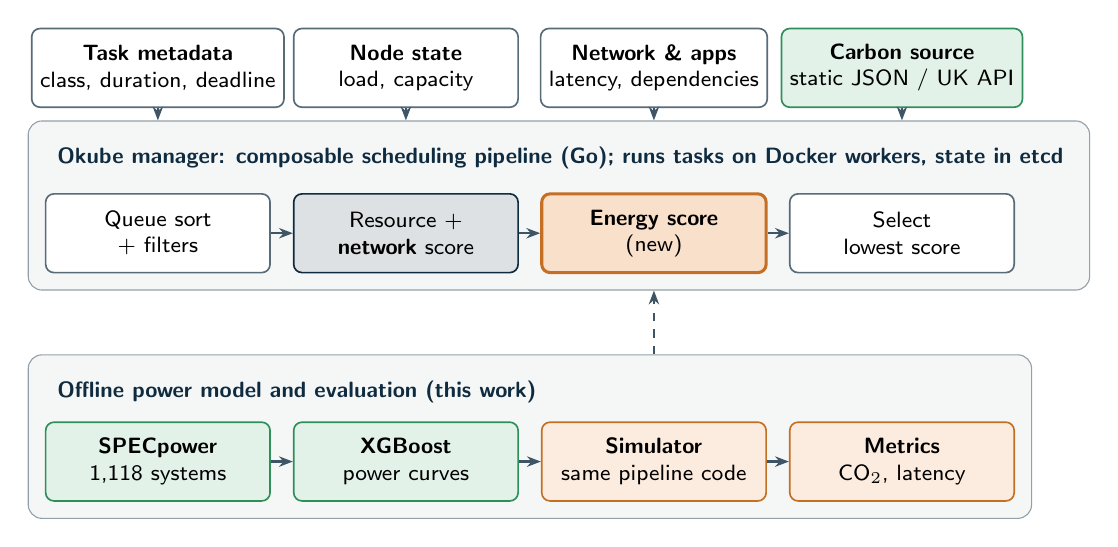
\begin{tikzpicture}[
  font=\sffamily\footnotesize,
  box/.style={draw=navy!70, rounded corners=3pt, fill=white, align=center, inner sep=3pt,
              line width=0.6pt, minimum height=1.0cm, minimum width=2.85cm},
  arr/.style={-{Stealth[length=5pt]}, line width=0.8pt, navy!80},
  darr/.style={arr, dashed},
  cont/.style={draw=navy!45, rounded corners=5pt, inner sep=6pt, fill=navy!4},
  title/.style={font=\sffamily\bfseries\footnotesize, navy, anchor=west},
]
\node[box] (in1) at (1.5,5.5)   {\textbf{Task metadata}\\class, duration, deadline};
\node[box] (in2) at (4.65,5.5)  {\textbf{Node state}\\load, capacity};
\node[box] (in3) at (7.8,5.5)   {\textbf{Network \& apps}\\latency, dependencies};
\node[box, fill=mint, draw=okgreen] (in4) at (10.95,5.5) {\textbf{Carbon source}\\static JSON / UK API};

\node[box] (p1) at (1.5,3.4)  {Queue sort\\+ filters};
\node[box, fill=navy!14, draw=navy] (p2) at (4.65,3.4) {Resource +\\\textbf{network} score};
\node[box, fill=okorange!25, draw=okorange!85!black, line width=1.1pt] (p3) at (7.8,3.4) {\textbf{Energy score}\\(new)};
\node[box] (p4) at (10.95,3.4) {Select\\lowest score};
\foreach \a/\b in {p1/p2,p2/p3,p3/p4}{\draw[arr] (\a) -- (\b);}
\node[title] (pt) at (0.1,4.35) {Okube manager: composable scheduling pipeline (Go); runs tasks on Docker workers, state in etcd};
\begin{scope}[on background layer]
  \node[cont, fit=(p1)(p4)(pt)] (pipe) {};
\end{scope}
\foreach \n in {in1,in2,in3,in4}{\draw[arr] (\n.south) -- (\n.south |- pipe.north);}

\node[box, fill=mint, draw=okgreen] (e1) at (1.5,0.5) {\textbf{SPECpower}\\1,118 systems};
\node[box, fill=mint, draw=okgreen] (e2) at (4.65,0.5) {\textbf{XGBoost}\\power curves};
\node[box, fill=okorange!15, draw=okorange!85!black] (e3) at (7.8,0.5) {\textbf{Simulator}\\same pipeline code};
\node[box, fill=okorange!15, draw=okorange!85!black] (e4) at (10.95,0.5) {\textbf{Metrics}\\CO$_2$, latency};
\foreach \a/\b in {e1/e2,e2/e3,e3/e4}{\draw[arr] (\a) -- (\b);}
\node[title] (et) at (0.1,1.38) {Offline power model and evaluation (this work)};
\begin{scope}[on background layer]
  \node[cont, fit=(e1)(e4)(et)] (evalc) {};
\end{scope}
\draw[darr] (e3.north |- evalc.north) -- (e3.north |- pipe.south);
\end{tikzpicture}
}
\end{center}
\end{frame}

% ------------------------------------------------------------------ 6 fused score
\begin{frame}[t]
\frametitle{The fused score}
\framesubtitle{Scheduling model}
\begin{columns}[T]
\begin{column}{0.56\textwidth}
\small
\textbf{Network cost} (Diktyo-style): summed latency to the nodes hosting a service's dependencies.\\[3pt]
\textbf{Carbon cost} on a fixed 0--100 scale:
\[ E(n,t)=100\,\min\!\Big(1,\tfrac{c_n}{0.3}\Big)\,\min\!\Big(1,\tfrac{L_{n,t}}{2}\Big) \]
$c_n$: carbon intensity (gCO$_2$/kWh$\,/1000$); $L_{n,t}$: load multiplier.\\[3pt]
\textbf{Class-aware weight and fused score:}
\[ w_e(t)=w\times\{0.35,\,1,\,1.4\},\qquad \mathrm{score}(n)=\mathrm{norm}(\mathrm{base})+w_e(t)\,E \]
\end{column}
\begin{column}{0.40\textwidth}
\begin{block}{Guarantees (all unit-tested)}
\small
\begin{itemize}
\item $w=0$ $\Rightarrow$ network-only, exactly
\item zero-carbon grid costs 0
\item unknown carbon uses a default
\item intensities above the reference saturate
\end{itemize}
\end{block}
\end{column}
\end{columns}
\end{frame}

% ------------------------------------------------------------------ 7 fixed scale
\begin{frame}[t]
\frametitle{Why a fixed scale: tiny gaps stay tiny}
\framesubtitle{Design finding}
\small
Energy cost assigned to three candidate grids (idle node, small task):
\begin{center}
\setlength{\tabcolsep}{7pt}
\begin{tabular}{@{}lcc@{}}
\toprule
Candidate grids (g/kWh) & Min--max normalised (first version) & Fixed scale (ours) \\
\midrule
0,\ 4,\ 15 \ \emph{(all very clean)} & 0,\ 27,\ 100 & \textbf{0,\ 0.7,\ 2.5} \\
0,\ 100,\ 237 \ \emph{(a real spread)} & 0,\ 42,\ 100 & \textbf{0,\ 17,\ 40} \\
\bottomrule
\end{tabular}
\end{center}
\begin{itemize}
\item The first version made a 15\,g/kWh node look as bad as possible next to a 0\,g/kWh node, so the scheduler would give up latency for a negligible carbon gain.
\item On a fixed scale the energy term only matters when the grids genuinely differ.
\item Found while testing against real data: the UK API reports exactly \textbf{0} for North Scotland, and the old code treated 0 as ``unset''.
\end{itemize}
\end{frame}

% ------------------------------------------------------------------ 8 data
\begin{frame}[t]
\frametitle{The data we use}
\framesubtitle{SPECpower\_ssj2008 and the UK Carbon Intensity API}
\begin{columns}[T]
\begin{column}{0.495\textwidth}
\begin{block}{SPECpower\_ssj2008 \ \chip{okgreen}{in results}}
\footnotesize
\begin{itemize}
\item Measured server power at \textbf{11 load levels} (idle, 10--100\%), published on spec.org.
\item \textbf{\NSystemsScraped{} detail pages} scraped, honouring the 10\,s crawl delay.
\item \NSystemsKept{} systems, \NRowsKept{} rows, \YearLo--\YearHi; multi-node systems divided per node.
\item \textbf{Use:} XGBoost $\rightarrow$ power curves $\rightarrow$ CO$_2$ in every result.
\end{itemize}
\end{block}
\end{column}
\begin{column}{0.495\textwidth}
\begin{block}{UK Carbon Intensity API \ \chip{okorange}{snapshot}}
\footnotesize
\begin{itemize}
\item NESO with Oxford, EDF Europe, WWF; \textbf{CC BY 4.0}; no API key.
\item Regional gCO$_2$/kWh for Great Britain, half-hourly, with a forecast.
\item Seen 23 Oct 2026: \textbf{0} (N.\ Scotland) to \textbf{237} (S.\ Wales).
\item \textbf{Use:} \texttt{fetch\_uk\_carbon.py} writes the manager's carbon file (real 0 kept); calibrates the simulated zones.
\item \textbf{Not yet:} continuous live refresh.
\end{itemize}
\end{block}
\end{column}
\end{columns}
\end{frame}

% ------------------------------------------------------------------ 9 power model
\begin{frame}[t]
\frametitle{Power model: watts from hardware and load}
\framesubtitle{Learned from SPECpower}
\begin{columns}[T]
\begin{column}{0.52\textwidth}
\begin{tikzpicture}
\begin{axis}[width=\textwidth, height=4.9cm, xlabel={CPU utilisation}, ylabel={Power (W)},
  xmin=0, xmax=1, ymin=0, grid=major, grid style={gray!25}, tick label style={font=\scriptsize},
  label style={font=\footnotesize}, legend style={font=\tiny, at={(0.03,0.97)}, anchor=north west}, legend cell align=left]
\addplot[thick, navy, mark=*, mark size=1.2pt] table[x=u, y=small] {generated/power_curves.dat};
\addlegendentry{8 cores (used)}
\addplot[thick, okgreen, mark=square*, mark size=1.2pt] table[x=u, y=mid] {generated/power_curves.dat};
\addlegendentry{32 cores}
\addplot[thick, okorange, mark=triangle*, mark size=1.5pt] table[x=u, y=large] {generated/power_curves.dat};
\addlegendentry{64 cores}
\addplot[thick, dashed, gray!70!black] table[x=u, y=placeholder] {generated/power_curves.dat};
\addlegendentry{old placeholder}
\end{axis}
\end{tikzpicture}
\end{column}
\begin{column}{0.45\textwidth}
\footnotesize
\resizebox{\linewidth}{!}{\begin{tabular}{@{}lrrrr@{}}
\toprule
 & \multicolumn{2}{c}{Grouped CV} & \multicolumn{2}{c}{Temporal split} \\
\cmidrule(lr){2-3}\cmidrule(lr){4-5}
Model & MAE & MAPE & MAE & MAPE \\
\midrule
Placeholder line (100--250\,W) & 142.5 & 65.1 & 250.8 & 65.9 \\
Line through true idle/max (oracle) & 20.5 & 7.7 & 33.7 & 8.2 \\
Ridge regression & 75.7 & 32.9 & 205.1 & 46.2 \\
XGBoost (ours) & 32.7 & 12.0 & 118.0 & 25.8 \\
\bottomrule
\end{tabular}
}
\vspace{4pt}
\begin{itemize}
\item XGBoost, monotone in load; scored on \textbf{held-out systems}.
\item Placeholder \MapePlaceholder\% error $\rightarrow$ model \MapeXgb\%.
\item A line through true idle/max: \MapeOracle\%.
\item Newer hardware is harder (\MapeTemporal\%).
\end{itemize}
\end{column}
\end{columns}
\end{frame}

% ------------------------------------------------------------------ 10 evaluation
\begin{frame}[t]
\frametitle{How we evaluate}
\framesubtitle{Simulator and protocol}
\begin{columns}[T]
\begin{column}{0.5\textwidth}
\small
\textbf{Simulator.} Seeded event loop driving the \emph{real} filter, score and select code; tasks queue when nodes are full.\\[3pt]
\textbf{Cluster.} 6 nodes (8 cores) in 3 zones: \texttt{scot} 50, \texttt{nw} 180, \texttt{south} 260 g/kWh (illustrative). The cleanest zone is the farthest from the dirtiest.\\[3pt]
\textbf{Workloads.} 60 app deployments, 20/40/40\% critical/flexible/default. \emph{Default}: $\sim$35\% utilisation. \emph{Stress}: 2.5$\times$ faster arrivals.
\end{column}
\begin{column}{0.47\textwidth}
\small
\textbf{Configurations.} default, network-only, energy-only, fused.\\[2pt]
\textbf{Metrics.} Dynamic CO$_2$, dependency latency, deadline violations, decision time.\\[2pt]
\textbf{Protocol.}
\begin{itemize}\footnotesize
\item paired: same trace per seed for every config
\item $w$ chosen on seeds 1--30 (largest within +10\% latency of network-only), so $w=\HeadlineW$
\item reported on \emph{disjoint} seeds 101--150 (\NSeeds{} runs), 95\% CIs
\end{itemize}
\end{column}
\end{columns}
\end{frame}

% ------------------------------------------------------------------ 11 results
\begin{frame}[t]
\frametitle{Result: less carbon, same latency win}
\framesubtitle{Default workload, \NSeeds{} held-out seeds}
\begin{columns}[c]
\begin{column}{0.60\textwidth}
\footnotesize
\resizebox{\linewidth}{!}{\begin{tabular}{@{}llrrrr@{}}
\toprule
Config & $w$ & CO$_2$ & $\Delta$CO$_2$ (\%) & Lat.\ (ms) & $\Delta$Lat.\ (\%) \\
\midrule
Default & -- & 25.66 & -- & 13.62 & -- \\
Network-only & -- & 25.20 & $-1.7\ \pm0.9$ & 2.26 & $-83.3$ \\
Energy-only & 0.2 & 24.91 & $-2.8\ \pm0.8$ & 11.82 & $-12.9$ \\
Fused & 0.2 & 24.32 & $-5.2\ \pm1.1$ & 2.09 & $-84.6$ \\
\midrule
Energy-only & 1.5 & 23.77 & $-7.3\ \pm0.8$ & 10.84 & $-20.2$ \\
Fused & 1.5 & 22.34 & $-12.9\ \pm1.2$ & 2.57 & $-81.0$ \\
\bottomrule
\end{tabular}
}\\[3pt]
{\tiny\color{navy!70} $\Delta$ vs default, paired; $\pm$ is a 95\% CI. Rows below the rule use $w=\HeadlineW$.}
\end{column}
\begin{column}{0.36\textwidth}
\centering
\stat{okorange}{$-$\FusedCO\%}{3.6cm}\\[1pt]{\scriptsize CO$_2$ vs default ($\pm\FusedCOci$)}\\[7pt]
\stat{okgreen}{$-$\FusedLatCut\%}{3.6cm}\\[1pt]{\scriptsize latency vs default\\(network-only: $-$\NetLatCut\%)}
\end{column}
\end{columns}
\vspace{5pt}
{\small Energy-only at the same weight: $-$\EnergyOnlyCO\% CO$_2$ but latency only $-$20\%. Under stress the carbon gain shrinks to $-$\FusedCOStress\%.}
\end{frame}

% ------------------------------------------------------------------ 12 tradeoff
\begin{frame}[t]
\frametitle{The weight trades carbon against latency}
\framesubtitle{Sweep over $w$}
\begin{columns}[T]
\begin{column}{0.60\textwidth}
\begin{tikzpicture}
\begin{axis}[width=\textwidth, height=5.8cm, xlabel={Mean dependency latency (ms)},
  ylabel={CO$_2$ reduction vs.\ default (\%)}, xmin=1.5, xmax=14.5, ymin=-3, ymax=46,
  grid=major, grid style={gray!25}, tick label style={font=\scriptsize}, label style={font=\footnotesize},
  legend style={font=\tiny, at={(0.98,0.97)}, anchor=north east}, legend cell align=left,
  every node near coord/.append style={font=\scriptsize, inner sep=1.5pt}]
\addplot[thick, okorange, mark=*, mark size=1.3pt] table[x=lat, y=red] {generated/sweep_fused_default.dat};
\addlegendentry{fused}
\addplot[thick, okgreen, mark=square*, mark size=1.3pt] table[x=lat, y=red] {generated/sweep_energyonly_default.dat};
\addlegendentry{energy-only}
\addplot[only marks, mark=diamond*, mark size=3pt, navy] table[x=lat, y=red] {generated/points_default.dat};
\addlegendentry{default / network-only}
\addplot[only marks, mark=*, mark size=1.3pt, okorange, nodes near coords, point meta=explicit symbolic, every node near coord/.append style={anchor=west, xshift=2pt, text=okorange!70!black}] table[x=lat, y=red, meta=label] {generated/labels_fused_default.dat};
\addplot[only marks, mark=square*, mark size=1.3pt, okgreen, nodes near coords, point meta=explicit symbolic, every node near coord/.append style={anchor=south west, text=okgreen!60!black}] table[x=lat, y=red, meta=label] {generated/labels_energyonly_default.dat};
\end{axis}
\end{tikzpicture}
\end{column}
\begin{column}{0.37\textwidth}
\small
\begin{itemize}
\item Fused sits far left of energy-only: same carbon, a fraction of the latency.
\item Labels give $w$; we pick $\mathbf{\HeadlineW}$ by a 10\% latency budget.
\item A looser budget picks a larger $w$ (about 35\% CO$_2$ at $w=5$).
\end{itemize}
\vspace{2pt}
{\scriptsize\textbf{By class} (fused, $w=\HeadlineW$): flexible $\rightarrow$ 119\,g/kWh nodes (default 162), critical $\rightarrow$ 183.}
\end{column}
\end{columns}
\end{frame}

% ------------------------------------------------------------------ 13 limits
\begin{frame}[t]
\frametitle{What the results do not show}
\framesubtitle{Threats to validity}
\small
\begin{itemize}
\item \textbf{Fused vs.\ energy-only is not a pure fusion test:} fused down-weights load balancing (0.3), energy-only does not.
\item \textbf{The learned model only counts CO$_2$;} placement uses the heuristic score.
\item \textbf{Carbon is illustrative and static.} Absolute CO$_2$ is relative, not real emissions; no time-shifting.
\item \textbf{Simulation only:} topological latency, one scenario family, identical hardware, no live run.
\item \textbf{One non-federated power model:} \MapeXgb\% held-out error, \MapeTemporal\% on newer systems.
\item \textbf{Stress:} gains nearly vanish; deadlines do not separate configs.
\end{itemize}
\end{frame}

% ------------------------------------------------------------------ 14 future
\begin{frame}[t]
\frametitle{Where this goes next}
\framesubtitle{Future work}
\begin{columns}[T]
\begin{column}{0.48\textwidth}
\begin{itemize}\small
\item \textbf{Live UK carbon feed} with the static file as offline fallback.
\item \textbf{Temporal placement}: use the forecast to delay flexible jobs into cleaner windows.
\item \textbf{Predicted watts in the score} instead of the load heuristic.
\end{itemize}
\end{column}
\begin{column}{0.48\textwidth}
\begin{itemize}\small
\item \textbf{Federated power model}, as in Saad et al.
\item \textbf{Fair ablation and a live multi-worker run.}
\item \textbf{Kubernetes Scheduling Framework port.}
\end{itemize}
\end{column}
\end{columns}
\end{frame}

% ------------------------------------------------------------------ 15 conclusion
\begin{frame}[t]
\frametitle{Conclusion}
\framesubtitle{Summary}
\begin{itemize}
\item One pipeline scores nodes on \textbf{network and carbon} cost, class-aware and independently switchable.
\item A \textbf{fixed-scale carbon cost} and a \textbf{power model learned from \NSystemsKept{} real servers} make the evaluation honest.
\item At $w=\HeadlineW$: \textbf{$-$\FusedCO\% CO$_2$} with latency still \textbf{\FusedLatCut\% below default}, which neither network-only nor energy-only reaches.
\item Limits are clear: simulation, illustrative carbon, one hardware type, saturated load.
\end{itemize}
\vspace{10pt}
\begin{center}{\Large\bfseries\color{navy} Thank you \ $\bullet$ \ Questions?}\end{center}
\end{frame}

\end{document}
